\documentclass[11pt,a4paper,titlepage]{article}
\usepackage[utf8]{inputenc}
\usepackage{amsmath}
\usepackage{amsfonts}
\usepackage{amssymb}
\usepackage{makeidx}
\usepackage{graphicx}
\usepackage{float}
\usepackage[T1]{fontenc}
\usepackage[usenames,dvipsnames]{xcolor}

\usepackage{pgf}
\usepackage{tikz}
\usetikzlibrary{arrows, automata, positioning, shapes, calc, trees, fit, scopes, chains}
%\usepackage{qtree}
\usepackage{tikz-qtree}
\usepackage{tikz-qtree-compat,textcomp}
\usepackage{tikz-dependency} % draw dependecy graphs

\depstyle{dep-style}{edge style = {thick, RoyalBlue,}, label style = {thick, text=RoyalBlue, fill=white, draw=RoyalBlue, font=\footnotesize, }, text style = {column sep=0.5cm, row sep=1ex,}, edge unit distance = 0.7em}
\depstyle{dep-style-narrow}{edge style = {thick, RoyalBlue},label style = {thick, text=RoyalBlue, fill=white, draw=RoyalBlue, font=\footnotesize,}, text style = {column sep=0.25cm, row sep=1ex}}

\tikzset{pattern-node/.style={
		rectangle,
		rounded corners,
		draw=black, very thick,
		minimum height=2em,
		inner sep=0.3em,
		text centered,
		align=center,
		node distance=3cm,
		anchor=center
	},
	pattern-node-negative/.style={
		rectangle,
		rounded corners,
		draw=black, very thick, dashed,
		minimum height=2em,
		inner sep=0.3em,
		text centered,
		align=center,
		node distance=3cm,
		anchor=center
	},
	edge-style/.style   = {very thick, ->,>=stealth, align=center,},
	tree-style/.style = {edge from parent fork down,
		edge from parent/.style={draw,rounded corners=3mm},
		edge-style,
		level 1/.style={sibling distance=10em},
		level 2/.style={sibling distance=10em}, level distance=7em},
	graph-style/.style = {sibling distance = 5em}
}
\tikzset{
	rect/.style n args={4}{
		draw=none,
		rectangle,
		append after command={
			\pgfextra{%
				\pgfkeysgetvalue{/pgf/outer xsep}{\oxsep}
				\pgfkeysgetvalue{/pgf/outer ysep}{\oysep}
				\def\arg@one{#1}
				\def\arg@two{#2}
				\def\arg@three{#3}
				\def\arg@four{#4}
				\begin{pgfinterruptpath}
					\ifx\\#1\\\else
					\draw[draw,#1] ([xshift=-\oxsep,yshift=+\pgflinewidth]\tikzlastnode.south east) edge ([xshift=-\oxsep,yshift=0\ifx\arg@two\@empty-\pgflinewidth\fi]\tikzlastnode.north east);
					\fi\ifx\\#2\\\else
					\draw[draw,#2] ([xshift=-\pgflinewidth,yshift=-\oysep]\tikzlastnode.north east) edge ([xshift=0\ifx\arg@three\@empty+\pgflinewidth\fi,yshift=-\oysep]\tikzlastnode.north west);
					\fi\ifx\\#3\\\else
					\draw[draw,#3] ([xshift=\oxsep,yshift=0-\pgflinewidth]\tikzlastnode.north west) edge ([xshift=\oxsep,yshift=0\ifx\arg@four\@empty+\pgflinewidth\fi]\tikzlastnode.south west);
					\fi\ifx\\#4\\\else
					\draw[draw,#4] ([xshift=0+\pgflinewidth,yshift=\oysep]\tikzlastnode.south west) edge ([xshift=0\ifx\arg@one\@empty-\pgflinewidth\fi,yshift=\oysep]\tikzlastnode.south east);
					\fi
				\end{pgfinterruptpath}
			}
		}
	},
	unit/.style={rect={draw=black, thick}{draw=black, thick}{draw=black, thick}{}},
	place/.style = {rect={draw=black, thick}{}{draw=black, thick}{draw=black, thick}, text width=5.5em,},
}
\tikzset{unt/.style={
		rectangle,
		rounded corners,
		draw=black, %very thick,
		minimum height=2em,
		inner sep=0.3em,
		text centered,
		align=center,
%		node distance=3cm,
		anchor=center
	},
	elm/.style={
		ellipse,
		%rounded corners,
		draw=black, dashed,% very thick, dashed,
%		minimum height=2em,
%		inner sep=0.3em,
		text centered,
		align=center,
%		node distance=3cm,
		anchor=center
	},
	fct/.style   = {dashed, ->,>=stealth, align=center,},
	cst/.style   = {->,>=stealth, align=center,},
}
\usepackage{tikz-uml}
\usepackage{gb4e} % for linguistic examples % let it be the last imported package to avoid exceeded parameter stack


%%%%%%%%%%%%%%%%%%%%%%%%%%%
\author{Eugeniu Costetchi}
\title{Conceptual analysis of several grammatical theories}
\begin{document}
\maketitle
\section{Introduction}
This paper sets to analyse the concepts used in several popular grammatical theories. The goal is to synthesize the all the concepts into a Generalized Annotation Model suitable for representing annotations and parses.

The models are OWL-DL compatible and expressed in UML graphical notation.

\section{Stanford dependency structure}
\label{sec:sds}
\begin{figure}[H]
	\centering
	\begin{dependency}[dep-style-narrow]
		\begin{deptext}[]
			NNP \& , \& WP \& VBZ \& VBG \& NN \& . \\
			Nina \& , \& who \& is \& coming \& tomorrow \& . \\ % \& , \& makes \& ... \\
		\end{deptext}
		\depedge[edge unit distance =2.2ex]{1}{5}{rcmod}
		\depedge{1}{3}{ref}
		\depedge{5}{3}{nsubjpass}
		\depedge{5}{4}{auxpass}
		\depedge{5}{6}{tmod}
	\end{dependency}
	\label{fig:dep1}
	\caption{Stanford dependency example}
\end{figure}

\subsection{Description of the concepts in use}
The parse structure is a graph. Nodes correspond to words and are connected by labelled edges. Some nodes that correspond to punctuation marks, prepositions or conjunctions are orphan and are not included in the connected graph of the sentence, even if they are instantiated. Edges are dependencies distilled in a fine grained typology. Each node beside the word literal carries: part of speech (POS), lemma, position in the sentence, and eventually the named entity (NE).

\subsection{Modelling Stanford dependency structure}

A minimal model of SD is represented in Figure \ref{fig:mode-dep-min} where nodes carry all the features as fixed set of attributes and have a dependecy relation to other nodes.

\begin{figure}[H]
	\centering
	\begin{tikzpicture}
	\umlclass[x=0]{Node}{word : Literal \\ lemma : Literal \\ id : Integer \\ pos : Literal \\ re : Literal}{}
	
	\umluniassoc[arg1=dependent, mult1=*, pos1=0.5,angle1=280, angle2=260, loopsize=1.5cm]{Node}{Node}
	\end{tikzpicture}
	\label{fig:mode-dep-min}
	\caption{Minial model for Stanford dependency structure}
\end{figure}

As an alternative, that would allow more flexibility in adding a unrestricted number of attributes on nodes would be to treat them as feature structures. A feature structure is a set of attribute value pairs where the attributes are strings representing a name and the values can be a data value (String, number, date, etc.) or another feature structure. 

Thus I propose to model the nodes as feature structures that contain several slots for each type of information: word, lemma, POS etc. However in order avoid mixing the relation types, it is still important to keep the node concept separated from the feature structure concept and treat the node as having an associated feature structure.

\begin{figure}[H]
	\centering
	\begin{tikzpicture}
	\umlclass[x=2]{Node}{}{}
	
	\begin{umlpackage}[x=3,y=0]{FM}
		\umlclass[x=4, y=0]{Feature Structure}{}{}
		\umlclass[x=4, y=-3]{Feature}{type : Literal \\ name : Literal \\ value : Literal}{}
	\end{umlpackage}
	
	\umluniassoc[arg1=features, mult1=1, pos1=0.5]{Node}{Feature Structure} %pos=0.8, 
	\umluniassoc[arg1=descendant, mult1=*, pos1=0.5]{Feature Structure}{Feature}
	\umluniassoc[arg1=descendant, mult1=*, pos1=0.5, angle1=100, angle2=80, loopsize=1.5cm]{Feature Structure}{Feature Structure}
	\umluniassoc[arg1=dependent, mult1=*, pos1=0.5,angle1=280, angle2=260, loopsize=1.5cm]{Node}{Node}
	\end{tikzpicture}
	\label{fig:mode-dep}
	\caption{Model of the Stanford dependency theory with feature structures}
\end{figure}

The edges or relations in the model are generalised under the \textit{dependent} relation. But in SG there is a whole taxonomy of relations. This is easy to model in OWL language but it is not easy to represent in UML diagram. When the formal model is created the \textit{dependent} relation shall be the root relation of the SD taxonomy, and the taxonomy itself shall be created in a separated ontology extending the current one. 

Actually, Stanford dependency becomes increasingly popular framework, and perhaps it shall be a part of the core model. The only problem is that there are other sets of dependency relations, for example those used by Malt parser, which are different from Stanford relations and they are school specific. 

\section{Word Grammar structure}
\label{sec:wgs}
Hudson's Word Grammar is a dependency grammar. It uses with a different set of word classes than Stanford grammar which relies on Penn POS set; it introduces the inflection features; and most importantly it distinguishes the order of the words by distinction \textit{post-dependent} and \textit{pre-dependent}. 

In Stanford Dependency the node order is indicated and controlled via the \textit{id} attribute which represents the order number of the node in the sentence. However in Word grammar, there is a specific mention of the order relation. This fundamental relation of node order is transitive and is modelled as in Figure \ref{fig:mode-dep-successor}

\begin{figure}[H]
	\centering
	\begin{tikzpicture}
	\umlclass[x=0]{Node}{}{}
	\umluniassoc[arg1=dependent, mult1=*, pos1=0.5,angle1=280, angle2=260, loopsize=1.5cm]{Node}{Node}
	\umluniassoc[arg1=successor, mult1=0..1, pos1=0.5,angle1=10, angle2=-10, loopsize=1.5cm]{Node}{Node}
	\end{tikzpicture}
	\label{fig:mode-dep-successor}
	\caption{Minial model of dependency node with a successor relation}
\end{figure}


One may argue that this is yet another typology of dependency relation and we shall not complicate the model. But if needed the \textit{successor} relation can be introduced and composed with \textit{dependent} relation in order to enforce the above distinction. The composition rules will then look like in \ref{ex:1} and \ref{ex:2}.
\begin{exe}
	\ex\label{ex:1} $pre\text{-}dependent(x,y) = dependent(x,y) \circ successor(y,x)$
	\ex\label{ex:2} $post\text{-}dependent(x,y) = dependent(x,y) \circ successor(x,y)$
\end{exe}

\section{Phrase structure}
\label{sec:ps}
In linguistics, phrase structure grammars are all those grammars that are based on the constituency relation, as opposed to the dependency relation associated with dependency grammars; hence phrase structure grammars are also known as constituency grammars.
\begin{figure}[H]
\centering
	\begin{minipage}{.45\textwidth}
		\centering
		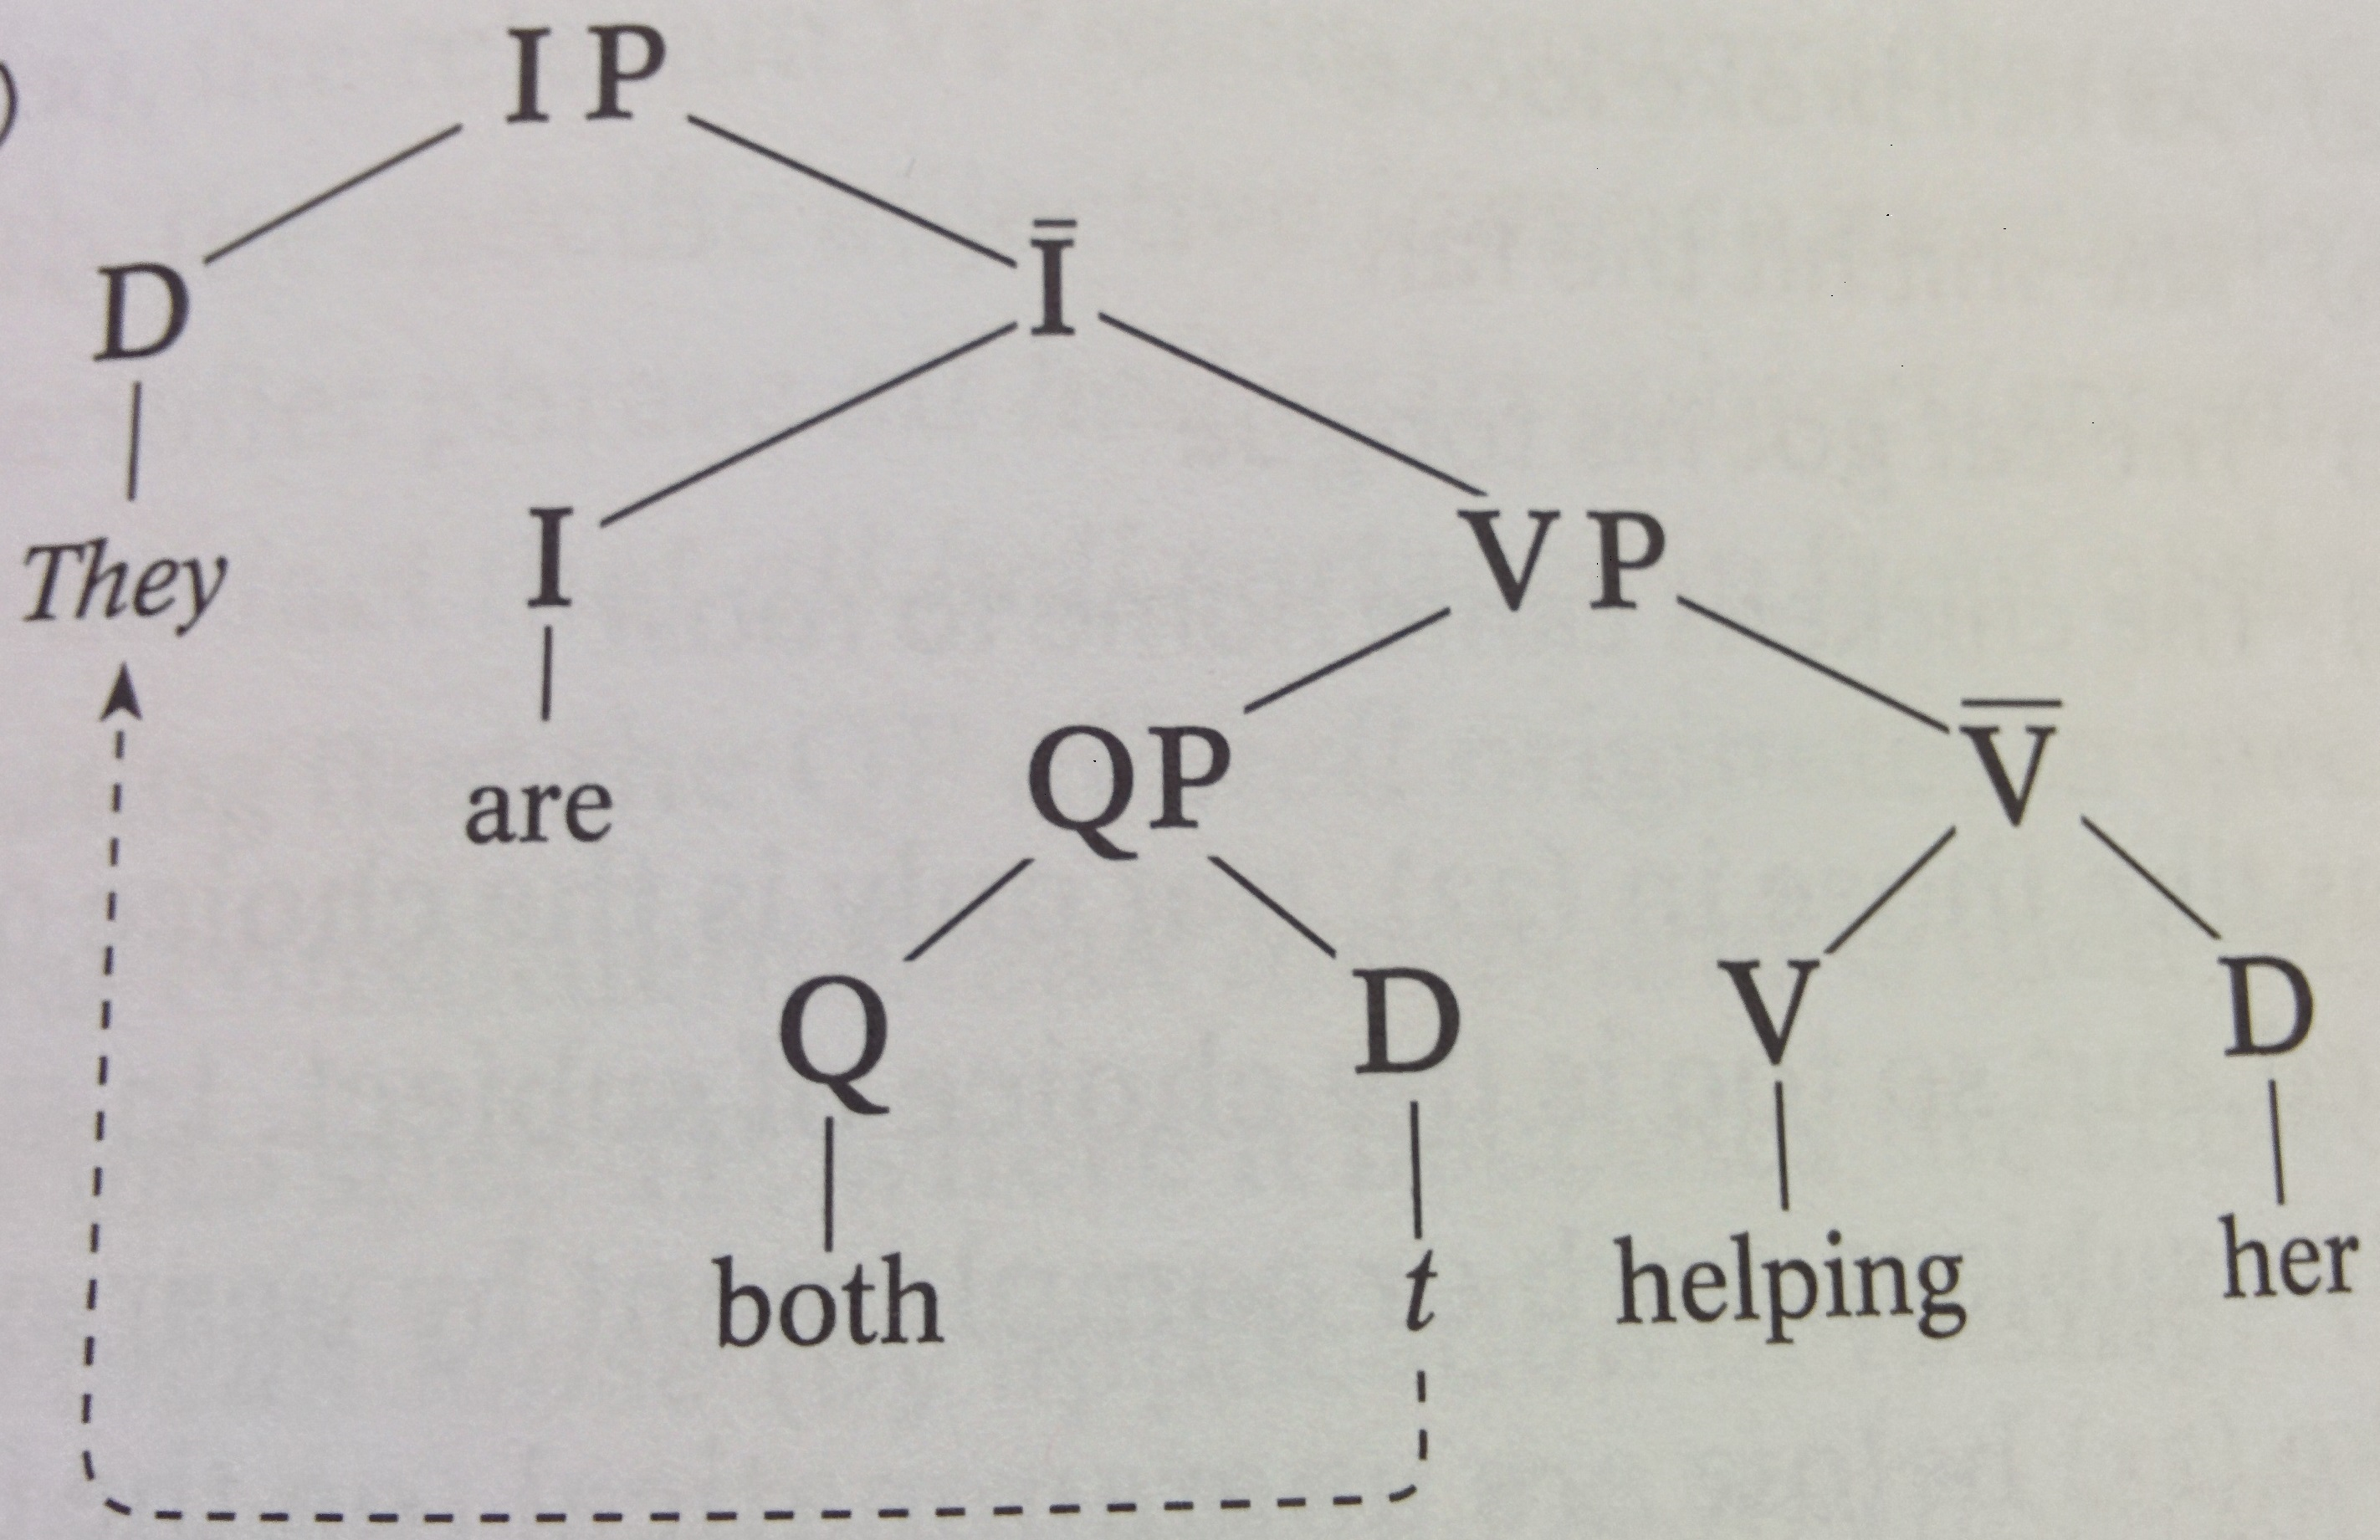
\includegraphics[width=\linewidth]{pics/tree1.jpg}
%		\label{fig:t1}
%		\caption{Phrase structure with a trace}
	\end{minipage}
	\begin{minipage}{.45\textwidth}
		\centering
		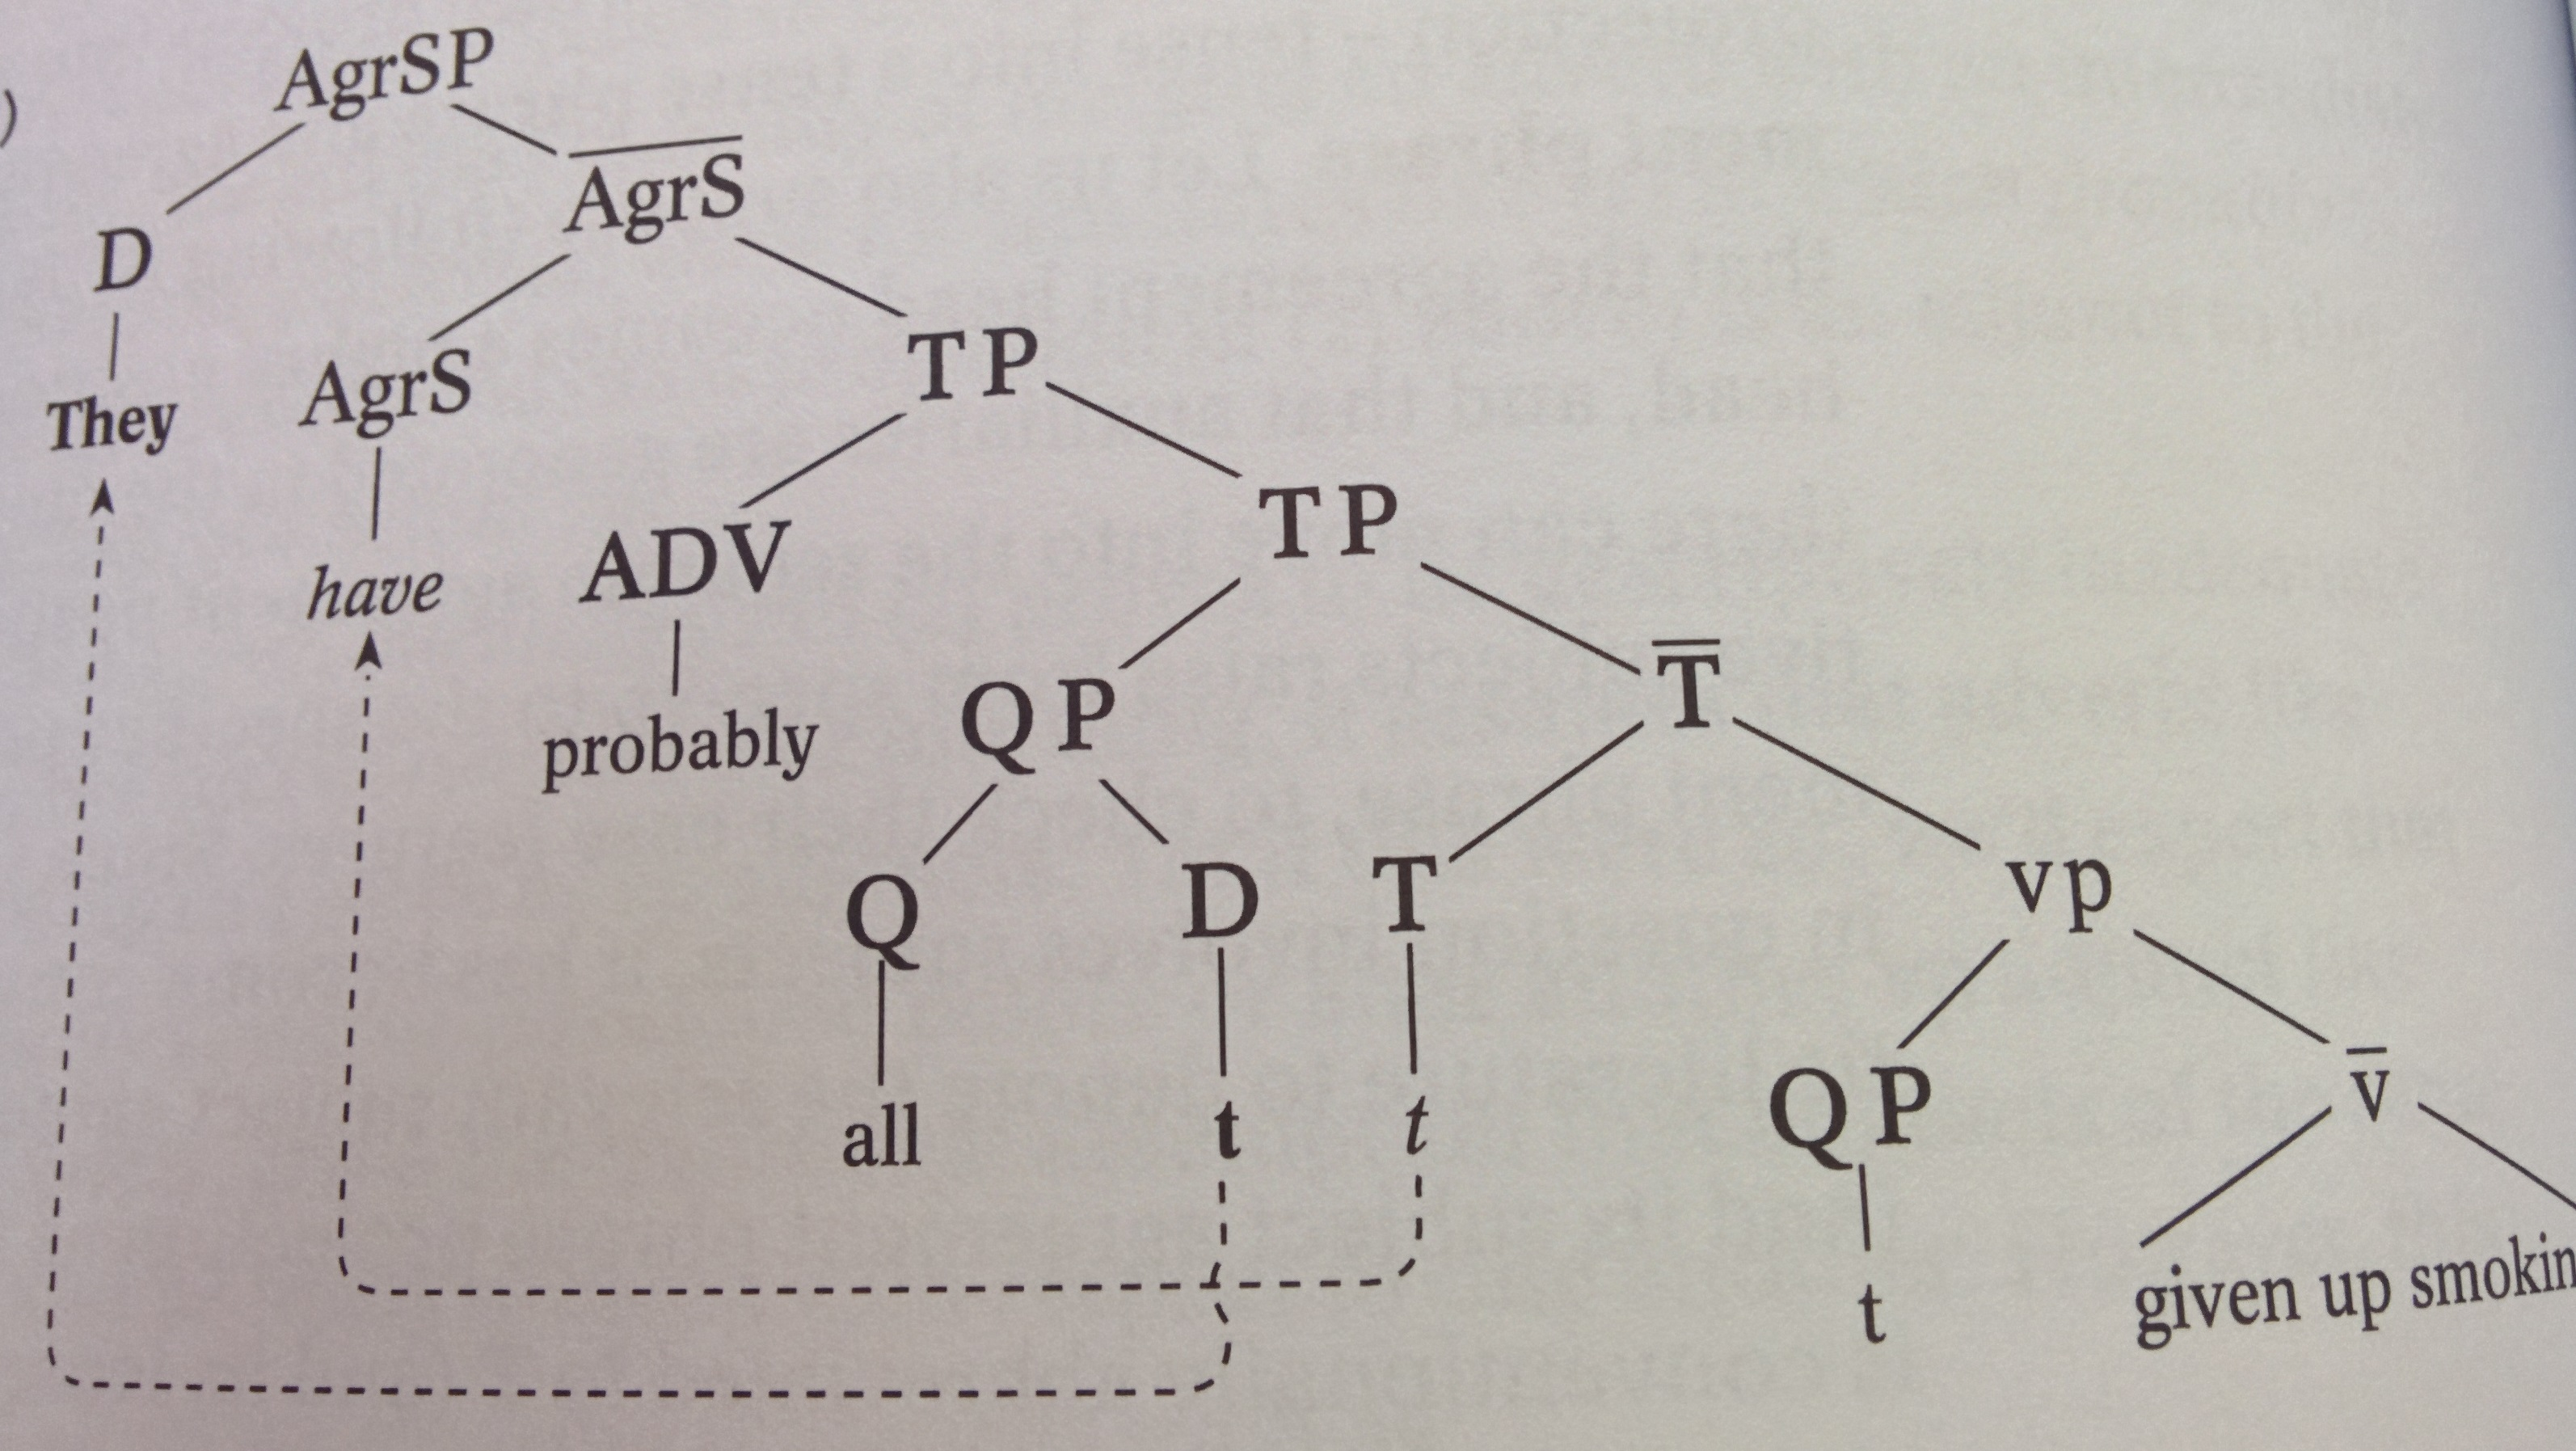
\includegraphics[width=\linewidth]{pics/tree2.jpg}
	\end{minipage}
	\caption{Phrase structure examples with traces}
\end{figure}

\subsection{Description of the concepts in use}
The phrase structure is a constituency structure represented as a tree. The tree nodes are either composite constituents or leaf nodes corresponding to words. The nodes usually represent the class of the constituent but may carry additional features, mainly agreement features, such as gender, number and case. Then the leaf nodes may correspond to a word, and empty constituent
Then there are trace elements, marked with \textit{t} or \textbf{t}, that result from either head (verb \& noun) movement or operator movement (aka wh-movement).

The edges of the tree are of only \textit{constituent} edges, where the parent node is composed of child nodes as parts. However there are also secondary secondary orthogonal relations for marking (a) movement and (b) agreement phenomena. The orthogonal edges can occur only between leaf nodes.

In the case of movement the relation stands between the trace and the moved element (or a transition trace).  Also depending on the type of movement, the traces and the moved element can (a) share all the features, (b) have distinct sets of features or (c) have a shared set and another non-shared set of features.

In the case of agreement the relation seems to play a similar role. This needs a further investigation because the meaning of agreement relation is different from the one representing movement. 

\subsection{Modelling phrase structure}
A model of phrase structure is presented in Lemon ontology \ref{} depicted in Figure \ref{fig:ps-lemon}. 

\begin{figure}[H]
	\centering
	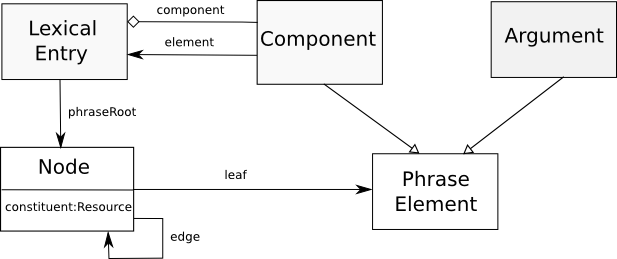
\includegraphics[width=\linewidth]{pics/lemon-ps-model}
	
	\caption{Phrase structure model in Lemon ontology}
	\label{fig:ps-lemon}
\end{figure}

Lemon model originated as a need to model lexical entries. Below in Figure \ref{fig:ps-model1}, I propose a model of phrase structure coming from the parsing and annotation direction. 

\begin{figure}[H]
	\centering
	\begin{tikzpicture}
		\umlclass[type=abstract, x=2, y=1]{Node}{}{}
		\umlclass[x=-1,y=-2]{Constituent Element}{}{}
		\umlclass[x=4,y=-2]{Leaf Element}{}{}
		\umlclass[x=1,y=-5]{Lexical Item}{}{}
		\umlclass[x=6,y=-5]{Null Element}{}{}
		\umlclass[x=7, y=1]{Feature Structure}{}{}
		
%		\umluniassoc[arg1=dependent, mult1=*, pos1=0.5,angle1=170, angle2=190, loopsize=1.5cm]{Node}{Node}
%		\umluniassoc[arg1=successor, mult1=0..1, pos1=0.5,angle1=10, angle2=-10, loopsize=1.5cm]{Node}{Node}
		\umlinherit[geometry=-|, anchor2=290]{Leaf Element}{Node}
		\umlinherit[geometry=-|, anchor2=250]{Constituent Element}{Node}
		\umlinherit[geometry=-|, anchor2=260]{Lexical Item}{Leaf Element}
		\umlinherit[geometry=-|, anchor2=280]{Null Element}{Leaf Element}
		
		\umluniassoc[geometry=|-, arg1=consistsOf, mult1=2, pos1=0.5 ]{Constituent Element}{Node}
		\umluniassoc[arg1=fills, mult1=1, pos1=0.5, angle1=220, angle2=190, loopsize=1.5cm ]{Leaf Element}{Leaf Element}
		
%		\umluniassoc[arg1=expected, mult1=1, pos1=0.5, anchor1=290, anchor2=north]{Leaf Element}{Null Element}
		
		\umluniassoc[arg1=agrees, mult1=1, pos1=0.5, angle1=170, angle2=190, loopsize=2cm]{Lexical Item}{Lexical Item}
		\umluniassoc[geometry=|-, arg1=traces, mult1=0..1, pos1=0.8, anchor1=30, anchor2=0]{Null Element}{Leaf Element}
		
		\umluniassoc[arg1=succeeds, mult1=0..1, pos1=0.5,angle1=120, angle2=60, loopsize=1.5cm]{Node}{Node}
		
		\umluniassoc[arg1=features, mult1=1, pos1=0.5]{Node}{Feature Structure}
	\end{tikzpicture}
	\caption{Phrase Structure Model}
	\label{fig:ps-model1}
\end{figure}

I distinguish between \textit{constituent} and \textit{leaf} nodes, which are either \textit{lexical items} of \textit{null elements}. The constituents must have two ordered children which can be either another constituent or a leaf node. The ordering of nodes I propose to model, just like in the case of Word Grammar (Section \ref{sec:wgs}), via \textit{successor} relation. Just like in the case of dependency grammar, the node class and any other features are organised in a feature structure. 

\begin{figure}[H]
	\centering
	\tikzstyle{every node}=[anchor=west]
	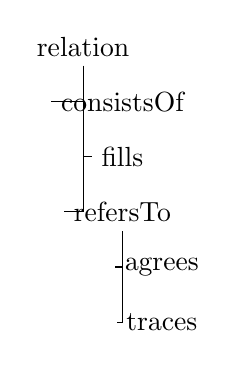
\begin{tikzpicture}[%
	grow via three points={one child at (0.5,-0.7) and
	two children at (0.5,-0.7) and (0.5,-1.4)},
	edge from parent path={(\tikzparentnode.south) |- (\tikzchildnode.west)}]
	\node{relation}
		child { node {consistsOf}}
		child { node {fills}}
		child { node {refersTo}
			child { node{agrees}}
			child { node{traces}} };
	\end{tikzpicture}
	\caption{Phrase structure relation taxonomy}
	\label{fig:ps-relation-taxnomy}
\end{figure}

The relation in phrase structure is also organised in a taxonomy as depicted in Figure \ref{fig:ps-relation-taxnomy}.

I did not consider for the moment semantic bindings PS. I do address though the syntax-semantics binding in the next section about Lexical Functional Syntax. 

\section{Lexical Functional Grammar}
Lexical Functional Grammar (LFG) is a type of generative phrase structure grammar. It is a reaction to the direction the transformational grammar was taking. It mainly focuses on syntax with relations to morphology and semantics. 

LFG views language as being made up of multiple dimensions of structure: argument, functional and categorial structures. Each of these dimensions, Figure \ref{fig:sfg-layers} is represented as a distinct structure with its own rules, concepts, and form. 

\begin{figure}[H]
	\centering
	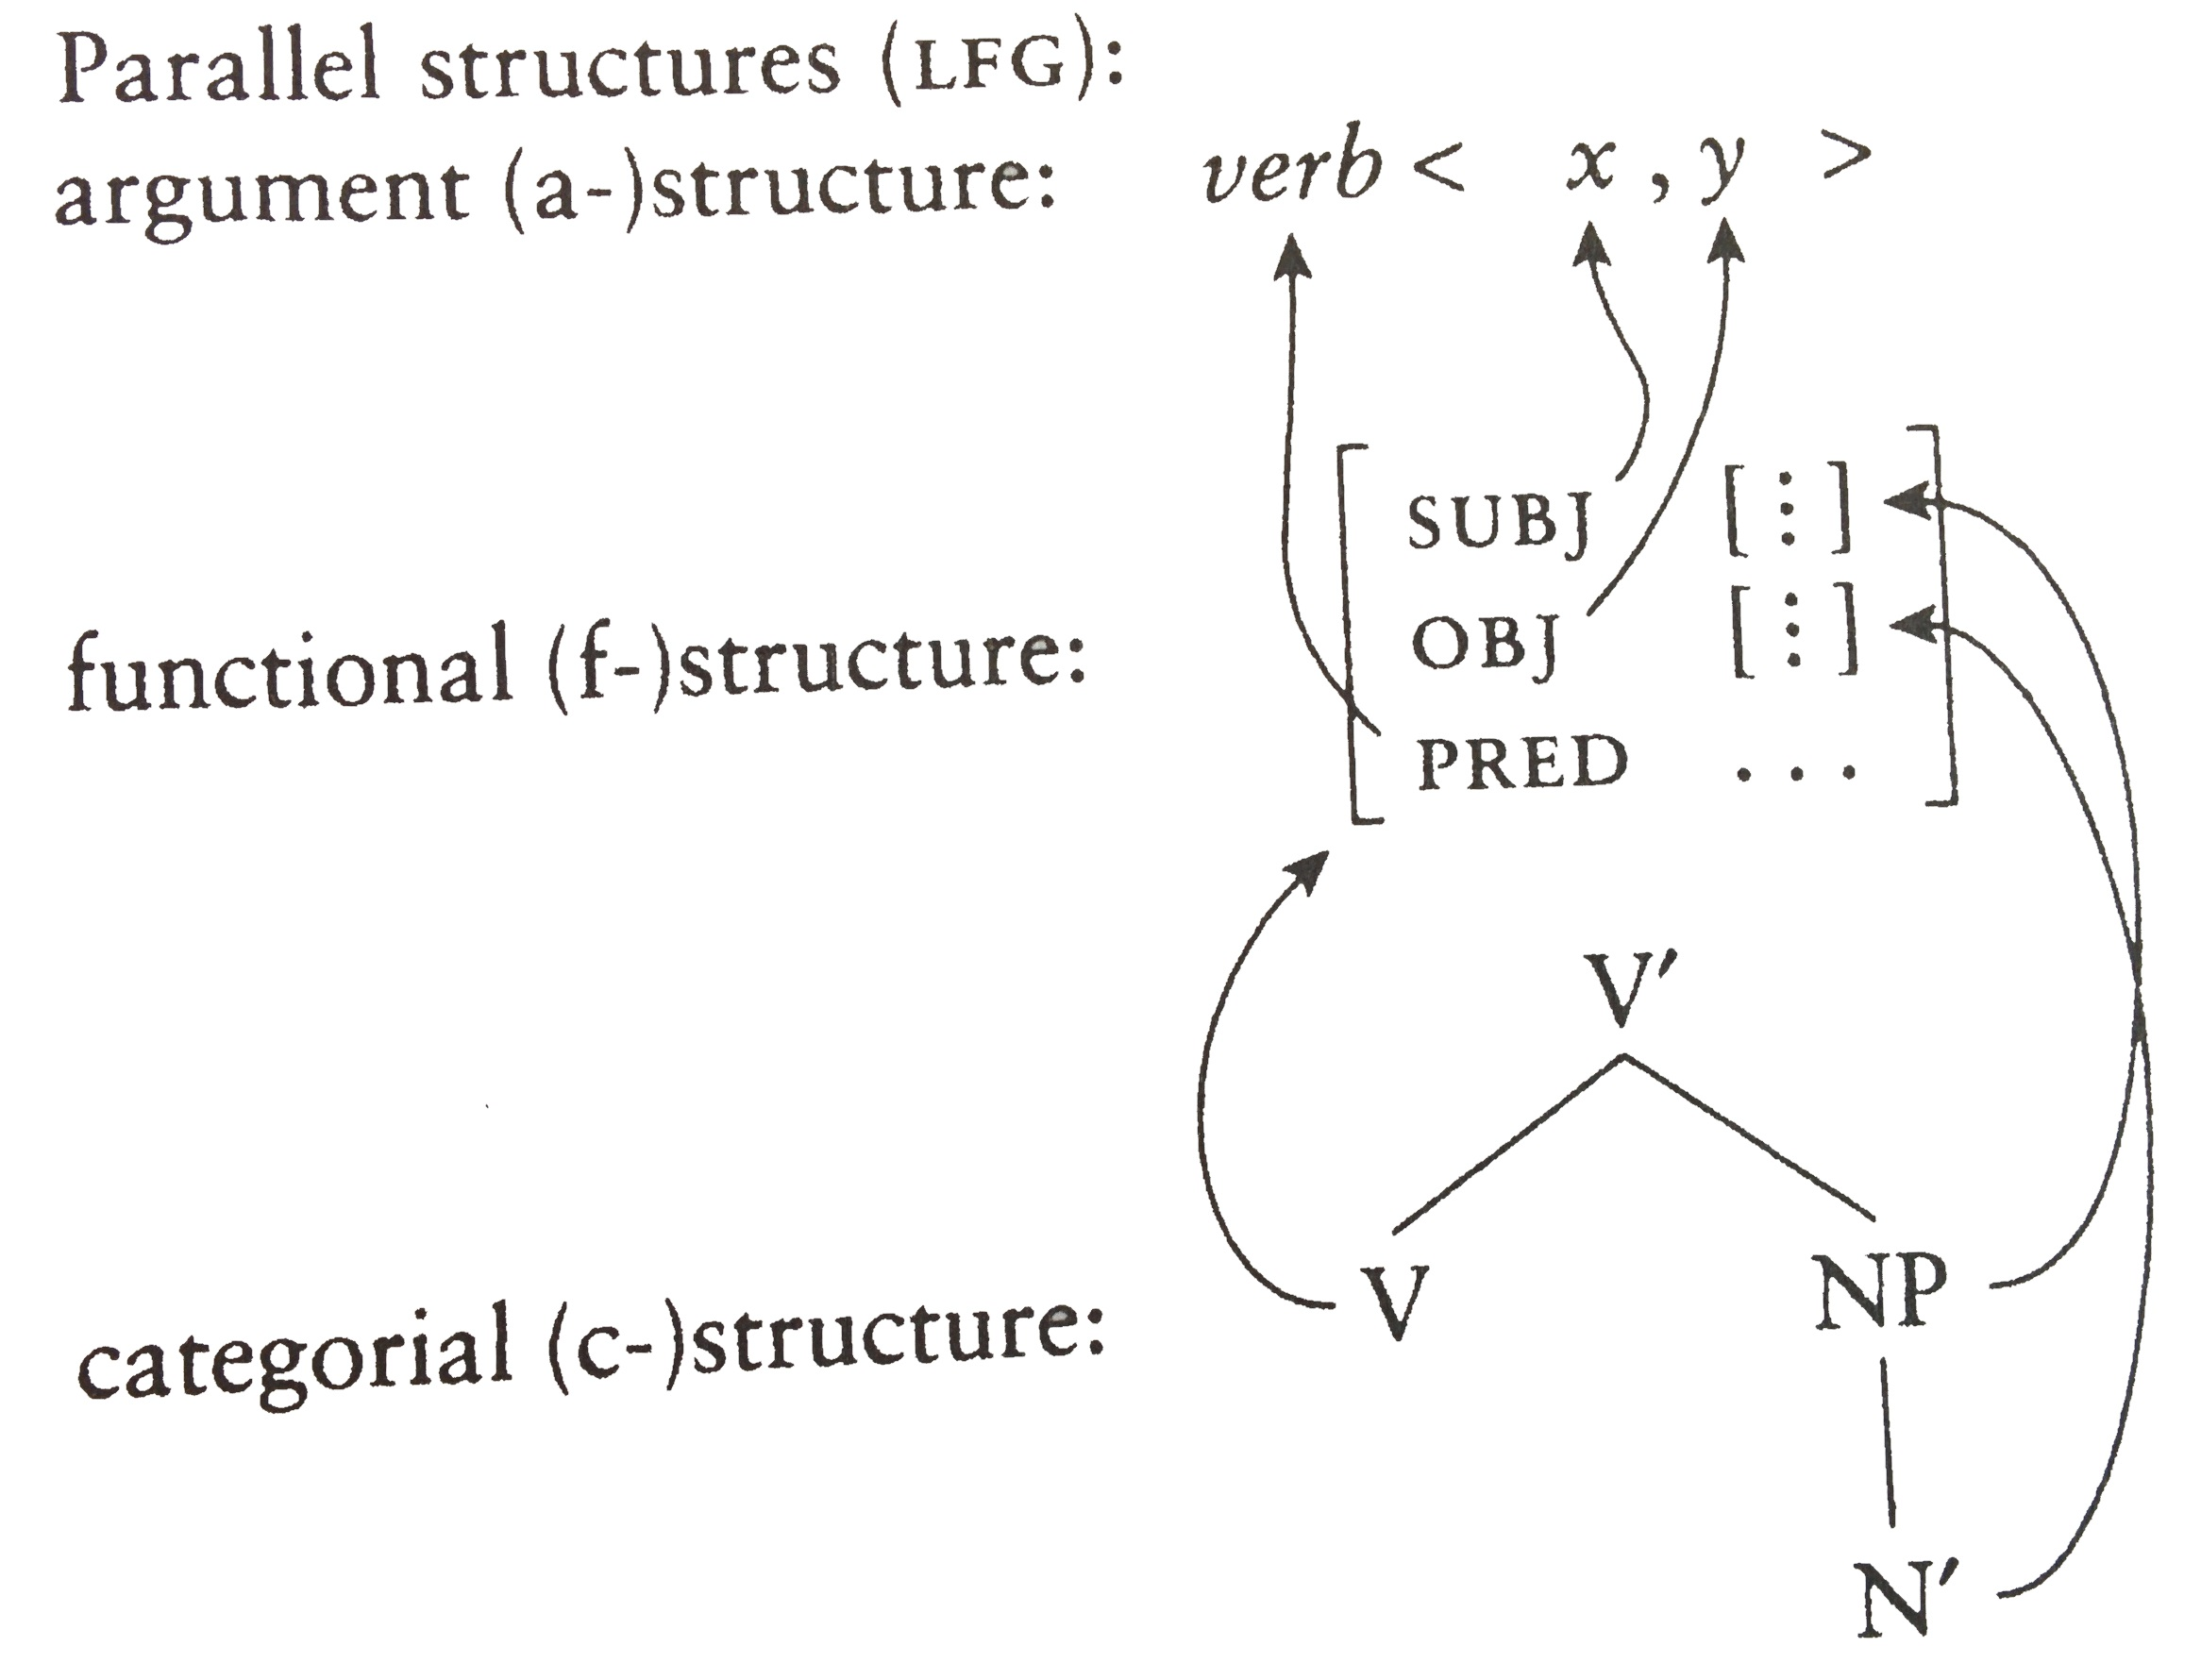
\includegraphics[width=0.6\linewidth]{pics/lfs-paralel-struct}
	\caption{SFG parallel structures}
	\label{fig:sfg-layers}
\end{figure}

\begin{figure}[H]
	\centering
	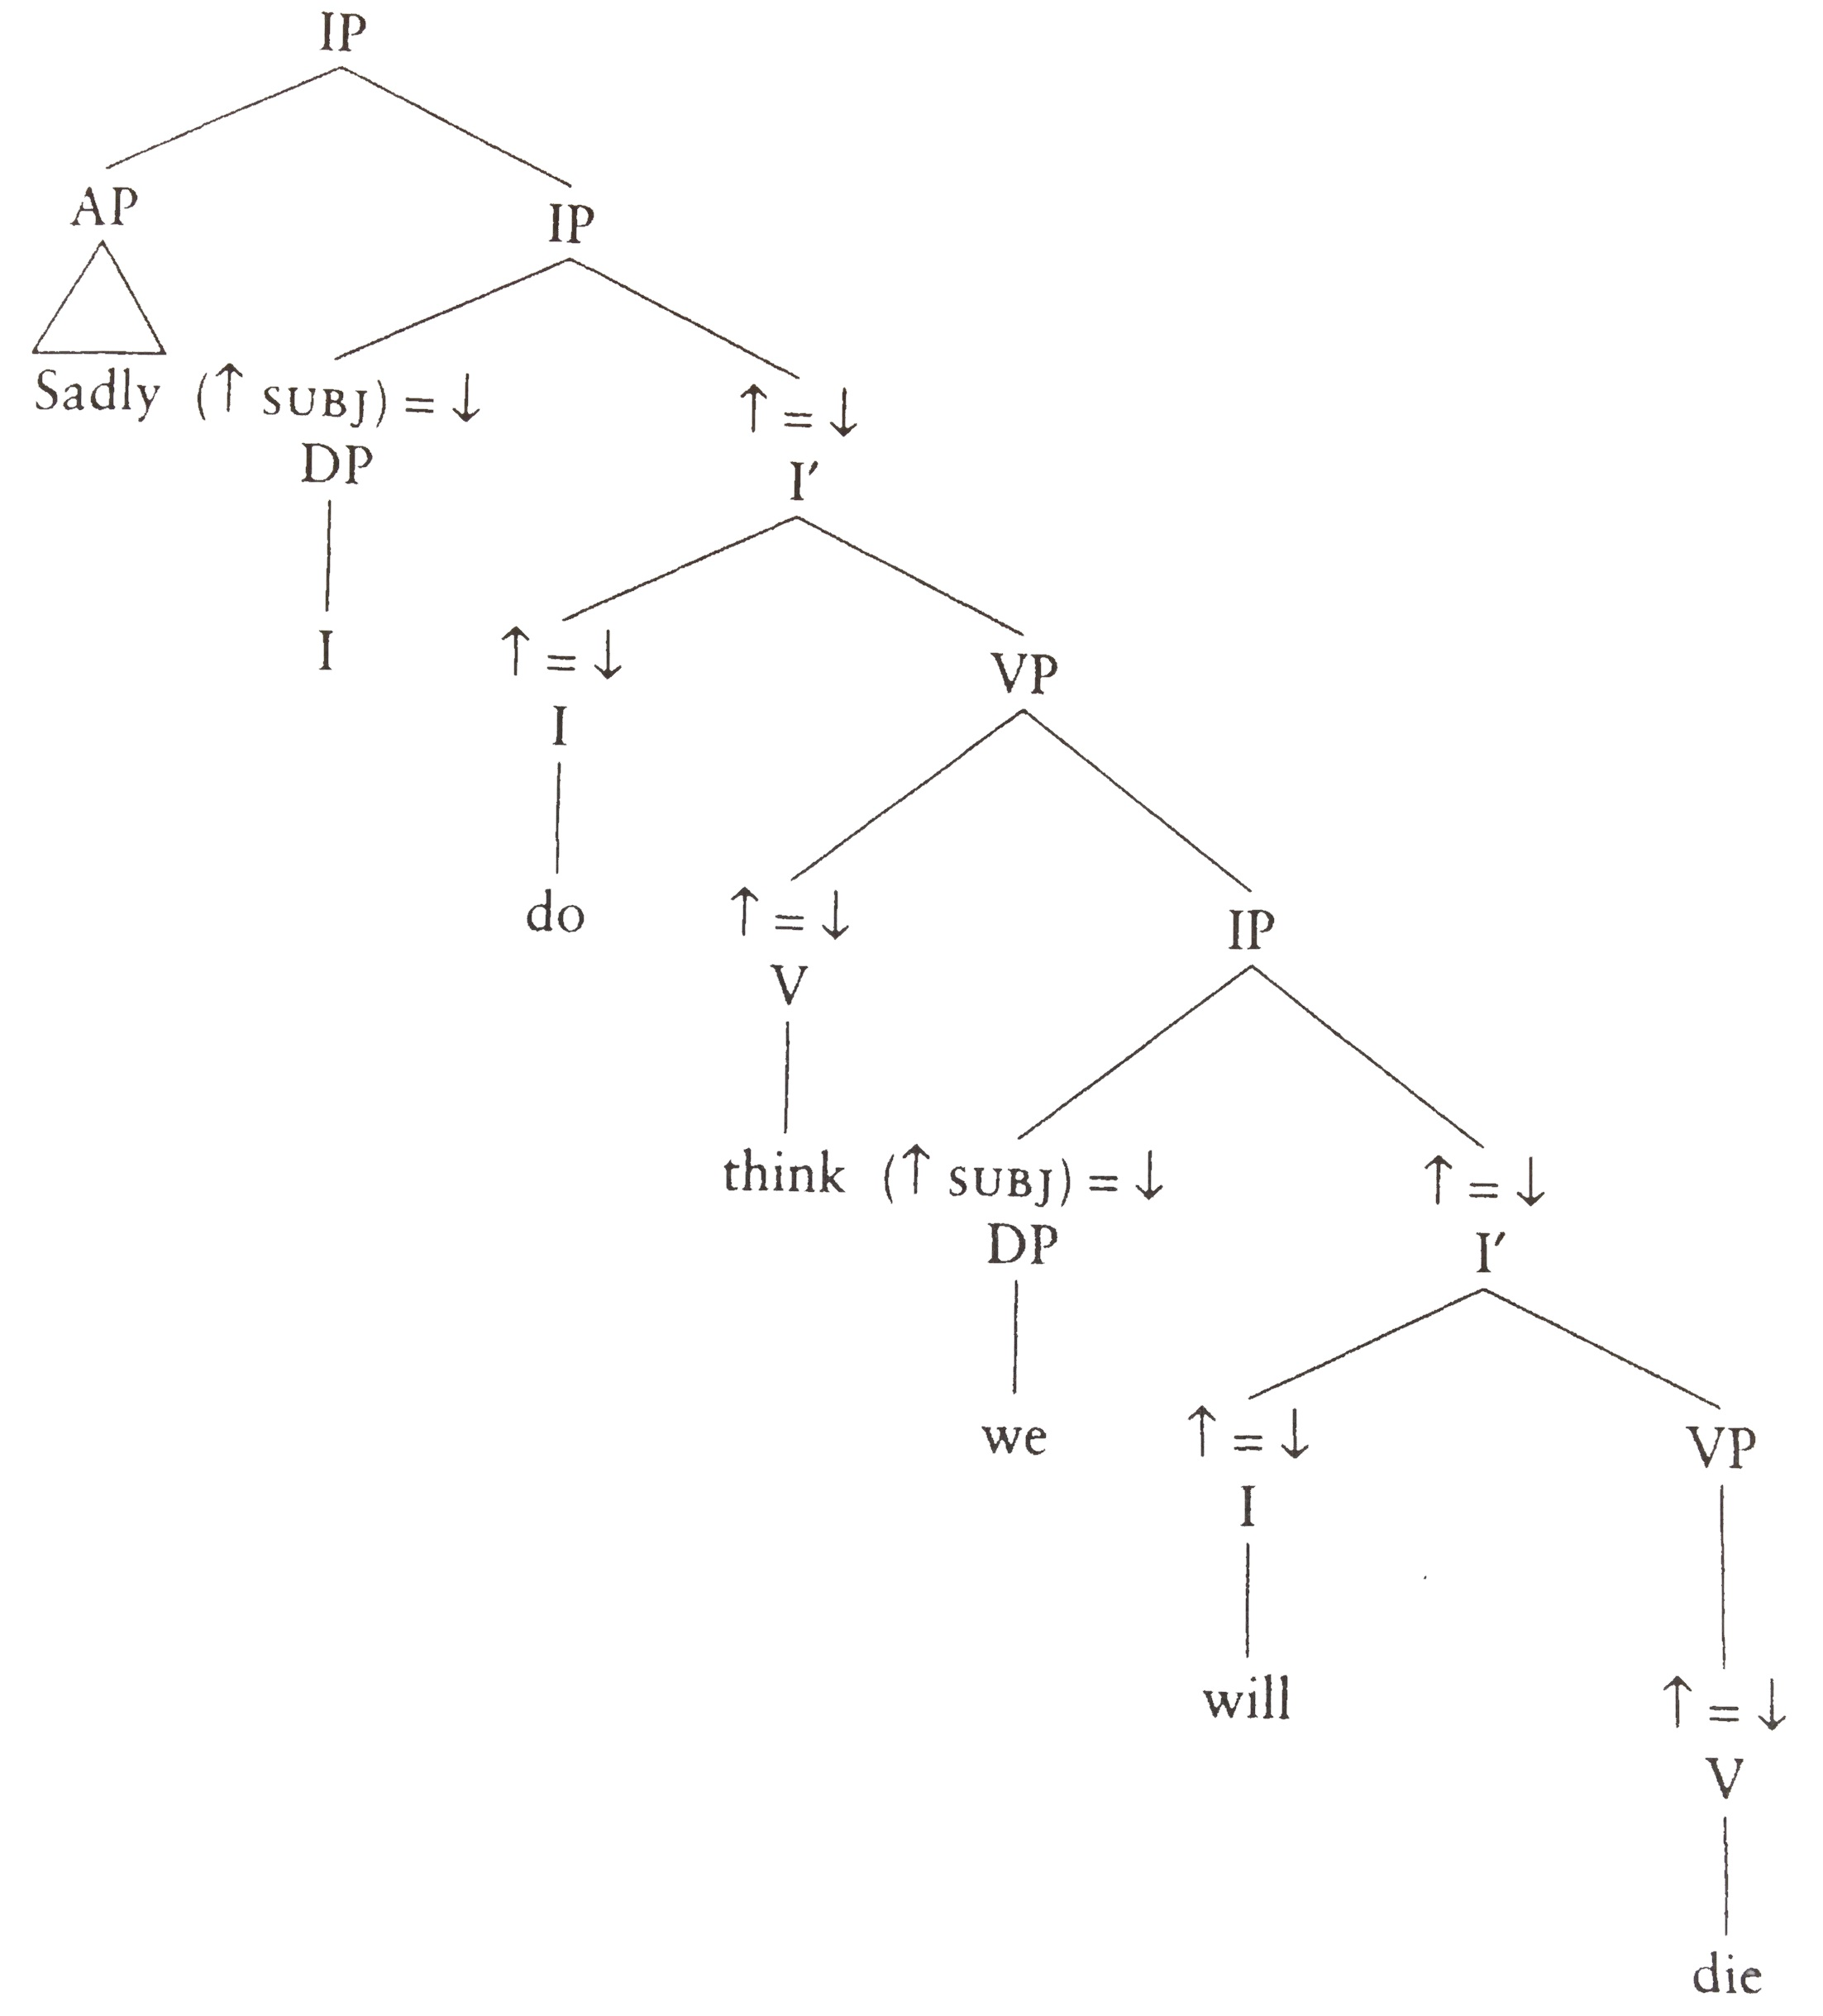
\includegraphics[width=0.6\linewidth]{pics/lfs-example2}
	\caption{SFG categorial structure with embedded functional markers}
	\label{fig:sfg-cstruct}
\end{figure}

\begin{figure}[H]
	\centering
	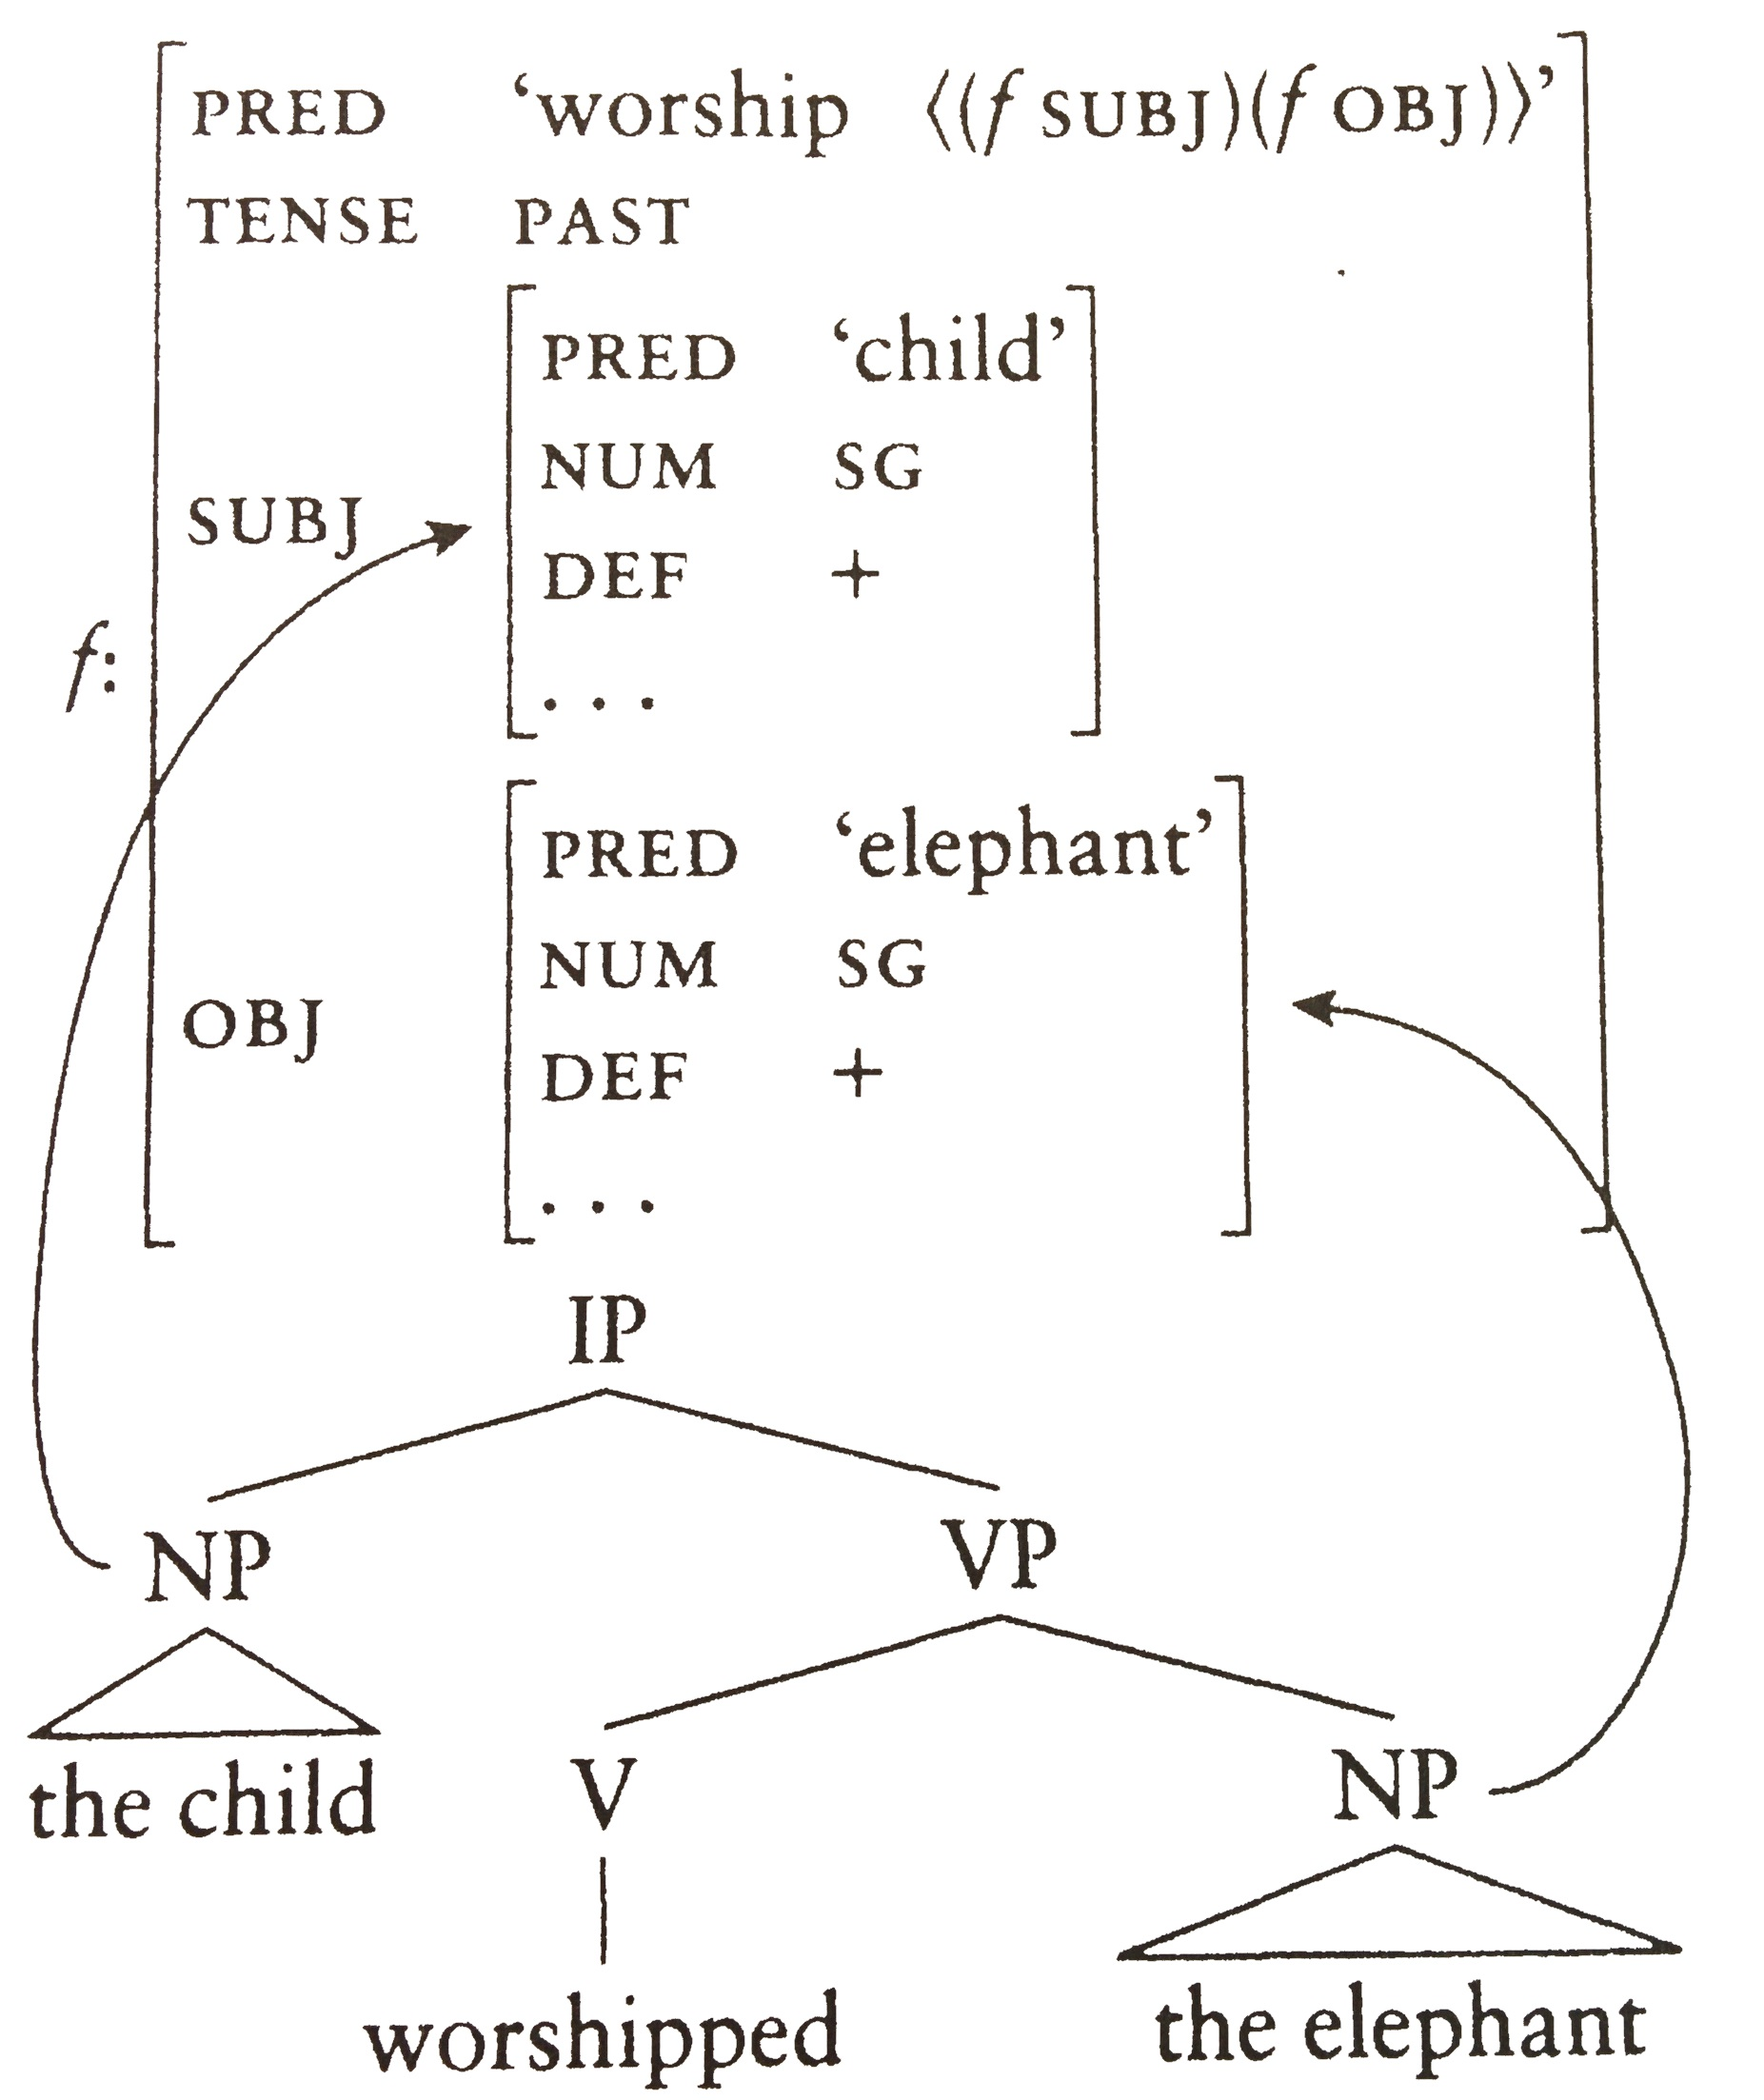
\includegraphics[width=0.6\linewidth]{pics/lfs-example1}
	\caption{SFG categorial structure mapped onto functional structure represented as feature structure}
	\label{fig:sfg-fstruct}
\end{figure}

The categorial structure is constituency based and is very similar to the phrase structure described in Section \ref{sec:ps}. The functional structure can be modelled as a feature structure described in the Section \ref{sec:sds}. 

\section{Systemic Functional meta model}

\begin{figure}[h]
	\begin{tikzpicture}
	
	\node[unit, text width=\textwidth,align=center](unit-line){};
	\node[above = 0.1em of unit-line](unit-label){Unit};
	%place lines
	{[start chain=l going left,node distance=1em]
		\node[on chain=l,place, below =3em of unit-line](p1){};
		\node[on chain=l,place](p2){};
		\node[on chain=l,place](p3){};
	}
	%place lines to the right
	{[start chain=r going right, node distance=1em,]
		\node[on chain=r,place, right = 1em of p1.east](p4){};
		\node[on chain=r,place](p5){};
	}
	%place labels
	\node[below=0.1em of p1](l3){place_{3}};
	\node[below=0.1em of p2](l2){place_{2}};
	\node[below=0.1em of p3](l1){place_{1}};
	\node[below=0.1em of p4](l4){place_{4}};
	\node[below=0.1em of p5](l5){place_{5}};
	%functional elements
	\node[above = 0.4em of p1, align=center, rectangle, draw, thick,dashed](element1){functional\\element_{3}};
	\node[above = 0.4em of p2, align=center, rectangle, draw, thick,dashed](element2){functional\\element_{2}};
	\node[above = 0.4em of p3, align=center, rectangle, draw, thick,dashed](element3){functional\\element_{1}};
	\node[above = 0.4em of p4, align=center, rectangle, draw, thick,dashed](element4){functional\\element_{4}};
	\node[above = 0.4em of p5, align=center, rectangle, draw, thick,dashed](element5){functional\\element_{5}};
	%order relations
	\draw[bend right,<->,dashed]  (l1) to node [below] {order} (l2);
	\draw[bend right,<->,dashed]  (l2) to node [below] {order} (l3);
	\draw[bend right,<->,dashed]  (l3) to node [below] {order} (l4);
	\draw[bend right,<->,dashed]  (l4) to node [below] {order} (l5);
	\end{tikzpicture}
	\caption{The graphic representation of (unit) structure}
	\label{fig:structure-representation}
\end{figure}

\begin{figure}[H]
	\centering
	\begin{tikzpicture}
	\umlclass[x=0,y=1]{Unit}{}{}
	\umlclass[x=-4,y=-2]{Lexical Item}{}{}
	\umlclass[x=4, y=-2]{Composite}{}{}
	\umlclass[x=0,y=-6]{Functional Element}{}{}
	
	\umlinherit[geometry=-|,anchor1=155]{Composite}{Unit}
	\umlinherit[geometry=-|,anchor1=22]{Lexical Item}{Unit}
	
	\umluniassoc[geometry=|-,arg1=isComposedOf, mult1=2..*, pos1=0.5, anchor1=300, anchor2=-10 ]{Composite}{Functional Element}
	\umluniassoc[geometry=-|,arg1=1..1, mult1=composes, pos1=0.5, anchor2=240, anchor1=10 ]{Functional Element}{Composite}
	
	\umluniassoc[geometry=-|,arg1=fills, mult1=1..*, pos1=1.1, anchor1=180, anchor2=90 ]{Composite}{Functional Element}
	\umluniassoc[geometry=|-,arg1=1..1, mult1=isFilledBy, pos1=0.2, anchor2=200, anchor1=40 ]{Functional Element}{Composite}
	
	\umluniassoc[geometry=|-,arg1=expounds, mult1=1..*, pos1=0.5, anchor1=300, anchor2=170 ]{Lexical Item}{Functional Element}
	\umluniassoc[geometry=-|,arg1=1..1, mult1=isExpoundedBy, pos1=1.1, anchor2=220, anchor1=190 ]{Functional Element}{Lexical Item}
	
	\umluniassoc[geometry=|-,arg1=hasConstituent, mult1=2..*, pos1=0.5,]{Composite}{Unit}
	\end{tikzpicture}
	\caption{SFL theory of grammar: the meta model}
	\label{fig:cardiff-metamodel}
\end{figure}

isComposedOf == hasFunction

functionsAs == fills
isFilledBy == 

%TODO http://citeseerx.ist.psu.edu/viewdoc/download?doi=10.1.1.324.2917&rep=rep1&type=pdf
\subsection{Cardiff grammar: instantiation example}

\begin{exe}
	\ex two hundred books.
	\ex She took them in.
	\ex Ask for three croissants and some milk.
\end{exe}

\begin{figure}[h]
	\centering
	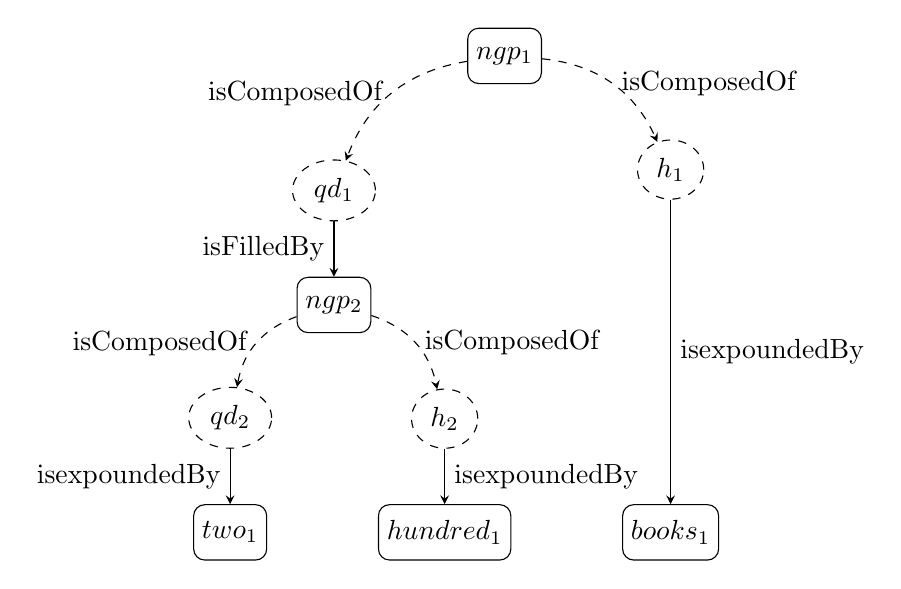
\begin{tikzpicture}
%	\node[unt,](clause1){clause1};
%	\node[elm, below = 2em of clause1,](subj1){subject1};
	
	\node[unt,](two){$two_1$};
	\node[unt, right =4em of two](hundred){$hundred_1$};
	\node[unt,right =4em of hundred](books){$books_1$};
	
	\node[elm,above =2em of two](qd2){$qd_2$};
	\node[elm,above =2em of hundred](h2){$h_2$};
	
	\node[unt,above =2em of h2, xshift=-4em](ngp2){$ngp_2$};
	\node[elm,above =2em of ngp2](qd1){$qd_1$};
	
	\node[elm,above =11em of books](h1){$h_1$};
	
	\node[unt,above =2em of h1,xshift=-6em](ngp1){$ngp_1$};
	
	%order relations
	\draw[fct,bend right,]  (ngp1) to node [left] {isComposedOf} (qd1);
	\draw[fct,bend left,]  (ngp1) to node [right] {isComposedOf} (h1);
	
	\draw[cst,]  (h1) to node [right] {isexpoundedBy} (books);
	\draw[cst,]  (qd1) to node [left] {isFilledBy} (ngp2);
	
	\draw[fct,bend right,]  (ngp2) to node [left] {isComposedOf} (qd2);
	\draw[fct,bend left,]  (ngp2) to node [right] {isComposedOf} (h2);
	
	\draw[cst,]  (qd2) to node [left] {isexpoundedBy} (two);
	\draw[cst,]  (h2) to node [right] {isexpoundedBy} (hundred);
	
%	\draw[bend right,<->,dashed]  (l3) to node [below] {order} (l4);
%	\draw[bend right,<->,dashed]  (l4) to node [below] {order} (l5);
	\end{tikzpicture}
	\caption{bla bla}
	\label{fig:example1}
\end{figure}

\subsection{Sydney grammar: instantiation example}

\end{document}